\documentclass{beamer}
\usepackage[utf8]{inputenc}
\usepackage{graphicx}

\usetheme{Madrid}
\usecolortheme{beaver}
% tira os trequinho feio de navegação
\title{VIM-de a mim, Produtividade}
\author{Gustavo Dutra}
\institute{http://gustavodutra.com}
\date{\today}
\begin{document}

\begin{frame}
\titlepage
\end{frame}

\begin{frame}{Sumário}
	\tableofcontents
\end{frame}

\section{Objetivo}
\begin{frame}{Objetivo}

Propor algumas práticas e repensar nossas ações a fim de torná-las mais eficazes e que consumam
menos tempo e esforço utilizando o \textbf{Vim} como editor de texto. Para isto, trago 3 princípios a serem 
seguidos e algumas soluções para os problemas que, pelo menos para mim, eram corriqueiros.

\end{frame}

\section{Vim}
\begin{frame}{Vim}
O Vim é um editor de texto e não, necessariamente, um editor de código-fonte.
Pode-se editar fácil e agilmente qualquer tipo de texto.
\begin{itemize}
	\item Posts de blogs
	\item E-mails
	\item Textos para wiki, fóruns, etc
	\item Posts de twitter
	\item Criar PDF's
	\item Criar apresentações
	\item <Insira sua idéia aqui>
\end{itemize}
\end{frame}

\section{Princípios}
\begin{frame}{Princípios}
São 3 os princípios para aumentar a produtividade, levando em conta a vontade
e a motivação para ser produtivo:
\begin{itemize}
	\pause \item \large Detectando problemas
	\begin{itemize}
		\item Erros constantes de digitação
		\item Trabalho manual desgastante
		\item Repetição de textos
	\end{itemize}
	\pause \item \large Procurando soluções
	\begin{itemize}
		\item Ler a documentação
		\item Procurar por plugins
		\item Procurar por dicas em blogs
		\item Criar um script em alguma linguagem
	\end{itemize}
	\pause \item \large Criando hábitos
	\begin{itemize}
		\item Refazer utilizando a solução
		\item Brincar com arquivos de testes
		\item Colar postit's no monitor
	\end{itemize}
\end{itemize}
\end{frame}

\section{Buscas}
\subsection{Importância}
\begin{frame}{Buscas - Importância}
	\begin{itemize}
		\item Certeza de encontrar todas as incidências
		\item Ficam visualmente destacadas (com :set hlsearch)
		\item Testar substituições
		\item Verificar a ortografia atrás de erros de digitação
		\item Encontrar variáveis ou funções não utilizadas, só declaradas
		\item Encontrar rapidamente algum termo
		\item Verificar a existência de algum termo
	\end{itemize}
\end{frame}

\subsection{Buscando com eficiência}
\begin{frame}{Buscando com eficiência}
	\begin{description}
		\item[/termo] Busca pela incidência de \textit{termo} nos arquivos abertos
		\item[:vimgrep] Abre os arquivos com a incidência do termo na Quickfix List
		\item[:vimgrepadd] Adiciona novos arquivos e incidências a Quickfix List
		\item[:grep] Executa um comando externo e abre os arquivos resultados (set grepprg)
		\item[:!grep] Apenas mostra o output do comando externo
	\end{description}
\end{frame}
\begin{frame}{/termo}
	\begin{block}{Exemplos}
	\begin{itemize}
		\item /texto
		\item /\textbackslash\textless{}casa\textbackslash\textless
		\item /\$var
		\item /public void static Main(String\textbackslash[\textbackslash] args)
		\item /\textbackslash{}([0-9]\textbackslash{}+\textbackslash{})texto\textbackslash{}1
	\end{itemize}
	\end{block}
	\begin{block}{Navegação}
	\begin{description}
		\item[n] Avança para a próxima incidência
		\item[N] Volta para a incidência anterior
		\item[zz] Centraliza a linha atual na tela
	\end{description}
	\end{block}
\end{frame}
\begin{frame}{:vimgrep}
	\begin{block}{:help :vimgrep}
		:vim[grep][!] /\{pattern\}/[g][j] \{files\}
	\end{block}
	\begin{itemize}
		\item Busca incidências de \textit{pattern} nos \textit{files} listados.
		\item \textit{pattern} pode ser uma expressão regular ou não
		\item A exclamação (\textit{!}) ignora as alterações já feita no arquivo atual
		\item \textit{g} procura por todas as incidências, não só a primeira, em cada arquivo
		\item \textit{j} pula para o primeiro resultado ao executar o comando
		\item \textit{files} podem conter \textit{wildcards}, como *, ? e **
		\item Os resultados são abertos na \textbf{quickfix list}
	\end{itemize}
\end{frame}
\begin{frame}{:vimgrep}
	\begin{block}{Exemplos}
	\begin{itemize}
		\item :vimgrep! /\$var/ arquivo.pl
		\item :vimgrep /texto/ *.rb
		\item :vimgrep /\textbackslash{}cTeXtO/ *.py dir/*.py
		\item :vimgrep /minhaFuncao/g **/*.c
		\item :vimgrep /\textless%
			\textbackslash{}([\textasciicircum{} ]\textbackslash+\textbackslash{})%
			[\textasciicircum{}\textgreater]*\textgreater.\textbackslash{}+%
			\textless\textbackslash{}/\textbackslash{}1\textgreater/ index.html
	\end{itemize}
	\end{block}
	\begin{block}{Navegando na Quickfix List}
	\begin{description}
		\item[:copen] Abre a Quickfix List
		\item[:cnext] Posiciona o cursor sobre a próxima incidência
		\item[:cprevious] Posiciona o cursor sobre a incidência anterior
		\item[:cclose] Fecha a Quickfix List
	\end{description}
	\end{block}
	% incluir screenshots =P
\end{frame}
\begin{frame}{:vimgrep}
	\begin{figure}[h!]
	  \caption{:vimgrep /:q\textbackslash{}>/g *tex}
	  \centering
	    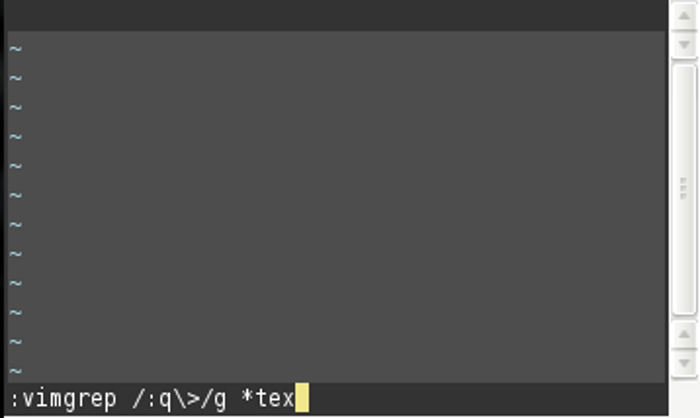
\includegraphics[width=0.7\textwidth]{sections/vimgrep/vimgrep1}
	\end{figure}
\end{frame}
\begin{frame}{:vimgrep}
	\begin{figure}[h!]
	  \caption{Resultado}
	  \centering
	    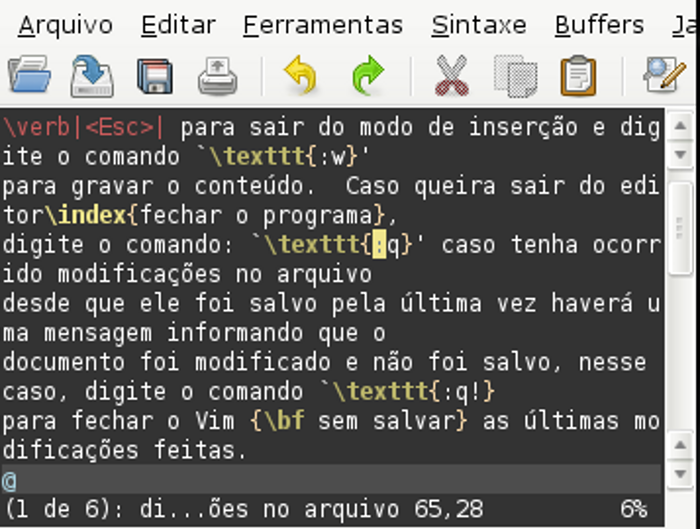
\includegraphics[width=0.7\textwidth]{sections/vimgrep/vimgrep2}
	\end{figure}
\end{frame}
\begin{frame}{:vimgrep}
	\begin{figure}[h!]
	  \caption{:copen}
	  \centering
	    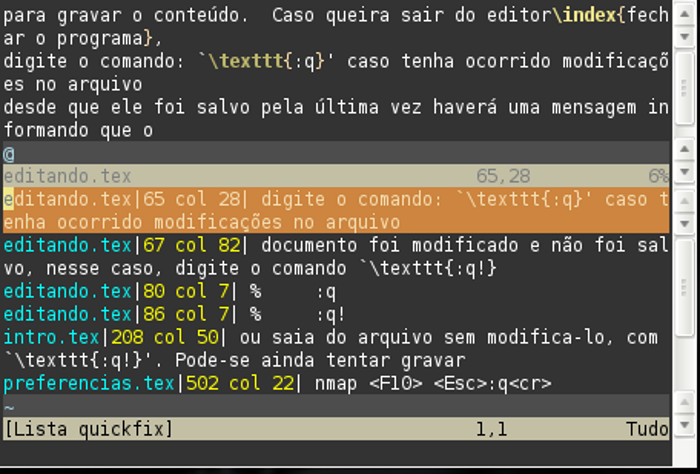
\includegraphics[width=0.7\textwidth]{sections/vimgrep/vimgrep3}
	\end{figure}
\end{frame}
\begin{frame}{:vimgrep}
	\begin{figure}[h!]
	  \caption{:cnext}
	  \centering
	    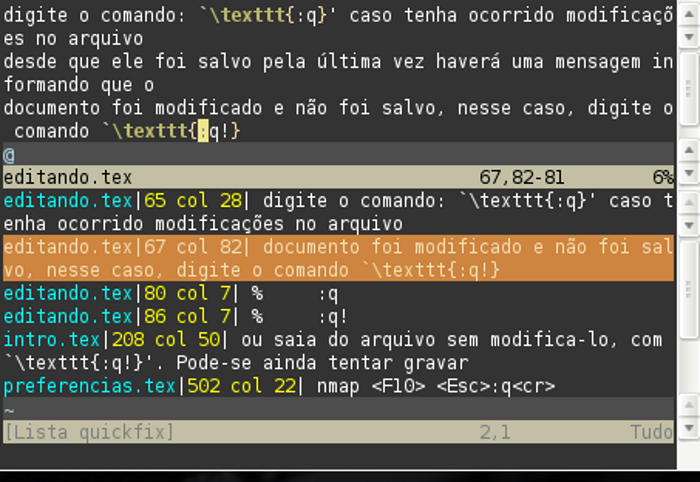
\includegraphics[width=0.7\textwidth]{sections/vimgrep/vimgrep4}
	\end{figure}
\end{frame}

\section{Operações em massa}
\begin{frame}{Operações em massa}
\begin{block}{Comandos}
	\begin{alert}{:bufdo cmd}
		Executa um comando em todos os buffers abertos (:e) \\
	\end{alert}
	:bfirst \\
	:cmd \\
	:bnext \\
	:cmd \\
	... \\
	\begin{alert}{:tabdo cmd}
		Executa um comandos em todas as abas abertas (:tabnew)\\
	\end{alert}
	:tabfirst \\
	:cmd \\
	:tabnext \\
	:cmd \\
	... \\
\end{block}
\end{frame}
\begin{frame}{Operações em massa}
\begin{block}{Comandos}
	\begin{alert}{:windo cmd}
		Executa um comandos em todas as janelas abertas (:[v]split)\\
	\end{alert}
	CTRL-w t \\
	:cmd \\ 
	CTRL-w w \\
	:cmd \\
	... \\
\end{block}
\end{frame}
\subsection{Exemplos}
\begin{frame}{Exemplos}
	\begin{itemize}
		\item :bufdo :\%s/\$variavel\_velha/\$variavel\_nova/g
		\item :bufdo :\%g/\textasciicircum\$/d
		\item :bufdo :\%g/\textasciicircum\#/d
		\item :tabdo :set fileencoding=utf-8 \textbar :w
		\item :bufdo :0r header.file
		\item :windo :syntax on \textbar :set syntax=tex
	\end{itemize}
\end{frame}

% não sei o que é \input{sections/list}
\section{Sessions}
\begin{frame}{Sessions}
	Imagine que você está em casa programando. Chega sua namorada e diz: "amor, desliga esse computador e vamos pro quarto". O que fazer?\\
	\pause \large Respostas:
	\begin{enumerate}
		\item Desliga o computador pressionando o botão pra ir mais rápido, mais tarde é só reabrir os arquivos e lembrar de onde parou
		\pause \item Diz pra ela que agora não pode, pois tem 10 arquivos abertos, 1 diff e está no meio de um algoritmo complexo
		\pause \item Finge que não escutou nada
		\pause \item Desliga o monitor e reza pra que ninguém mais mexa no computador
		\pause \item Salva a sessão e continua da onde parou quando quiser
	\end{enumerate}
\end{frame}
\begin{frame}{Sessions}
	Sempre que se abre o vim, se inicia uma nova sessão. E nela são gravados:
	\begin{itemize}
		\item Hitórico de comandos
		\item Históricos de \textit{undos}
		\item Arquivos abertos em buffers
		\item Arquivos abertos em abas
		\item Mapeamento de teclas
		\item Abreviaturas\ldots
	\end{itemize}
	\begin{block}{Como usar?}
		:mksession sessions/algoritmo\_X.vim \\
		\$ vim -S sessions/algoritmo\_X.vim
	\end{block}
\end{frame}

\section{Macros}
\begin{frame}{Macros}
	\begin{block}{Macro}
	\begin{itemize}
		\item Macro é um conjunto de comandos que podem ser executados automaticamente com uma finalidade.
		\item Geralmente são usadas para tarefas repetitivas e que seguem um padrão.
		\item Macros muito utilizadas podem ser carregadas automaticamente pelo \textbf{.vimrc}
	\end{itemize}
	\end{block}
	% exemplo de macro: ID;NOME criar uma query de update.
\end{frame}

\section{Pulos}
\begin{frame}{Pulos}
	\begin{description}
		\item[gg] Primeira linha do arquivo
		\pause \item[G] Última do arquivo 
		\pause \item[\textasciicircum] Primeiro caracter não nulo
		\pause \item[\$] Último caracter não nulo
		\pause \item[b] Primeiro caracter da palavra acima do cursor
		\pause \item[e] Última caracter da palavra acima do cursor
		\pause \item[fx] Primeira incidência depois do cursor de \textit{x} na linha
		\pause \item[Fx] Primeira incidência anterior ao cursor de \textit{x} na linha
	\end{description}
\end{frame}
\begin{frame}{Pulos por Marcas}
\begin{block}{Quando usar?}
	\begin{itemize}
		\item Quando se é difícil encontrar algum trecho específico do arquivo
		\item Quando se precisa apenas um trecho de vários arquivos pra se escrever um outro
		\item Quando o arquivo é muito longo e precisa ser scrollado
		\item \textless{}Insira aqui a sua utilidade\textgreater
	\end{itemize}
\end{block}
\end{frame}
\begin{frame}{Pulos por Marcas}
\begin{block}{Como usar?}
	\begin{description}
		\item[ma] Marca a letra \textit{a} neste ponto.
		\begin{itemize}
			\item Marca a linha cujo cursor está em cima.
			\item Pode-se utilizar qualquer uma das 26 letras.
			\item São 26 letras por arquivo aberto.
			\item Devem ser em minúsculas.
		\end{itemize}
		\item[mA] Marca a letra \textit{A} neste ponto.
		\begin{itemize}
			\item Marca a linha cujo cursor está em cima.
			\item Pode-se utiilziar qualquer uma das 26 letras.
			\item São 26 letras por sessão.
			\item Devem ser em minúsculas.
			\item São visíveis de qualquer arquivo
		\end{itemize}
		\item['a] Pula para a marca \textit{a} (mesmo arquivo)
		\item['A] Pula para a marca \textit{A} (mesma sessão)
	\end{description}
\end{block}
\end{frame}

\section{Abreviações}
\begin{frame}{Abreviações}
\begin{itemize}
	\item Corrigir frequêntes erros de digitação
	\item Correção gramatical
	\item Facilitar escrita de textos muitos longos
	\item Podem variar de acordo com tipo do arquivo (.txt, .java, .c)
	\item Exemplos:
	\begin{description}
		\item[pq] porque
		\item[tchelinux] Tche Linux - Rio Grande Do Sul
		\item[forloop] for (\$i = 0; \$i \textless count(\$array); \$i++) \{\}
		\item[:Wq] :wq
		\item[:Q] :q
	\end{description}
\end{itemize}
\end{frame}
\begin{frame}{Abreviações}
\begin{block}{Como usar?}
	\begin{itemize}
		\item :iabbr pq porque
		\item :iabbr tchelinux Tche Linux - Rio Grande Do Sul
		\item :abbr forloop for (\$i = 0; \$i \textless count(\$array); \$i++) \{\}
		\item :cabbr Wq wq
		\item :cabbr Q q
		\item{:cabbr trim s/\textasciicircum\textbackslash{}s\textbackslash{}+\textbar\textbackslash{}s\textbackslash{}+\$//g}
	\end{itemize}
\end{block}
\end{frame}

\section{Templates}
\begin{frame}{Templates}
	\begin{block}{Funcionalidade}
		Permite que, ao abrir um novo arquivo, o arquivo tenha um template padrão
		\begin{itemize}
			\item Acelerando o desenvolvimento
			\item Certificando-se de que não será esquecido de nada
			\item Menos erros de digitação
			\item Evita o raciocínio e a memorização sobre coisas desnecessárias
			\item Padroniza documentos
		\end{itemize}
	\end{block}
	\begin{block}{Utilidade}
		\begin{itemize}
			\item Criar template para uma extensão de arquivo
			\item Criar template para um arquivo que contenha uma certa palavra
			\item Criar template para um arquivo que esteja dentro de um certo diretório
		\end{itemize}
	\end{block}
\end{frame}

\subsection{Exemplos}
\begin{frame}{Exemplos}
	\begin{enumerate}
		\item Criar o arquivo bash.template com o template desejado
		\item Colocar no .vimrc o código para carregar o template para todos os arquivos com extensão .sh
		\item Sentir a magia
	\end{enumerate}
	\begin{block}{bash.template}
		\#!/bin/bash
	\end{block}
	\begin{block}{.vimrc}
		autocmd BufNewFile *.sh 0r bash.template
	\end{block}
	\begin{block}{Shell}
		\$ vim teste.sh
	\end{block}
\end{frame}

\section{Plugins}
\begin{frame}{Plugins}
\begin{itemize}
	\item NERDTree
	\item FuzzyFinder
	\item SnipMate
	\item PotWiki
	\item Taglist
	\item MiniBufExpl
	\item MatchIt %testar!
	\item Mark % testar!
	\item VimOutliner
\end{itemize}
\end{frame}

\section{Dúvidas}
\begin{frame}{Dúvidas}
	\begin{center}
		{\Huge Dúvidas?}
	\end{center}
	\begin{flushright}
		{\tiny Agradecimento especial Emanuel Zabka}
	\end{flushright}
\end{frame}


\end{document}
